\chapter{A Case study of legged locomotion}
\label{sec:casestudy}


\section{Requirement of legged locomotion}
\label{sec:case_req}

\subsection{Fast leg placement}
\label{sec:fast}

\subsection{Impact management}
\label{sec:impact}

\subsection{High load bearing}
\label{sec:load}


\section{Solution based on variable gear-ratio actuators}
\label{sec:case_sol}

\begin{figure}[H]
        \centering
				\subfloat[Fast leg placement]{
				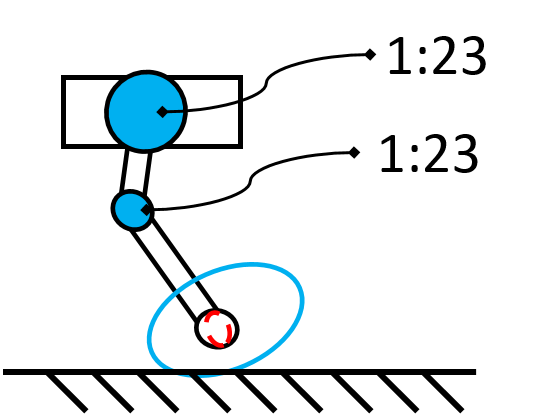
\includegraphics[width=0.35\textwidth]{legHS.png}
				\label{fig:legHS}}
        \subfloat[High load bearing]{
				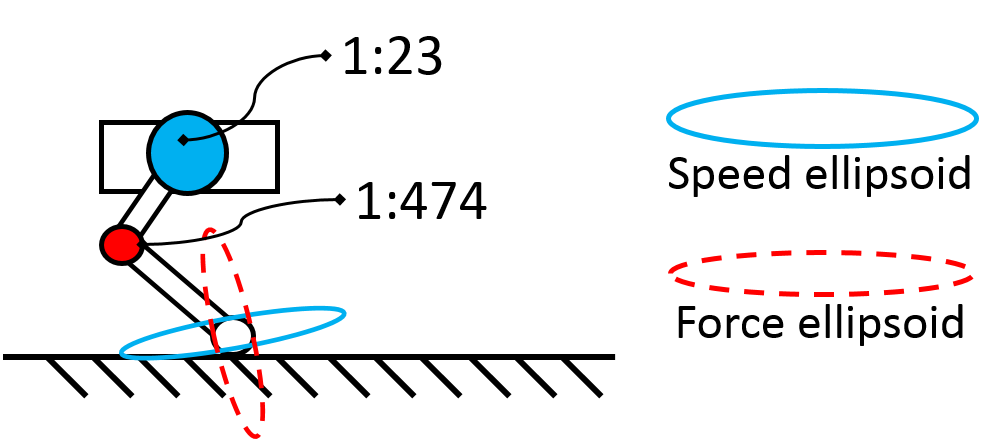
\includegraphics[width=0.65\textwidth]{legHF.png}
				\label{fig:legHF}}
        \caption{Advantageous gear-ratio selection for locomotion}\label{fig:legsol}
\end{figure}



\section{Case Study: 1-DoF leg landing}

\subsection{Modeling}

Fig. \ref{fig:1dof_landing} shows a rigid body dynamic model of the robot. This system has 3 DoF : absolute velocity of robot base $\dot{x}_R$, relative leg/actuator velocity $\dot{a}$ and internal DoF in the DSDM $w_1$. 

\begin{figure}[htp]
	\centering
		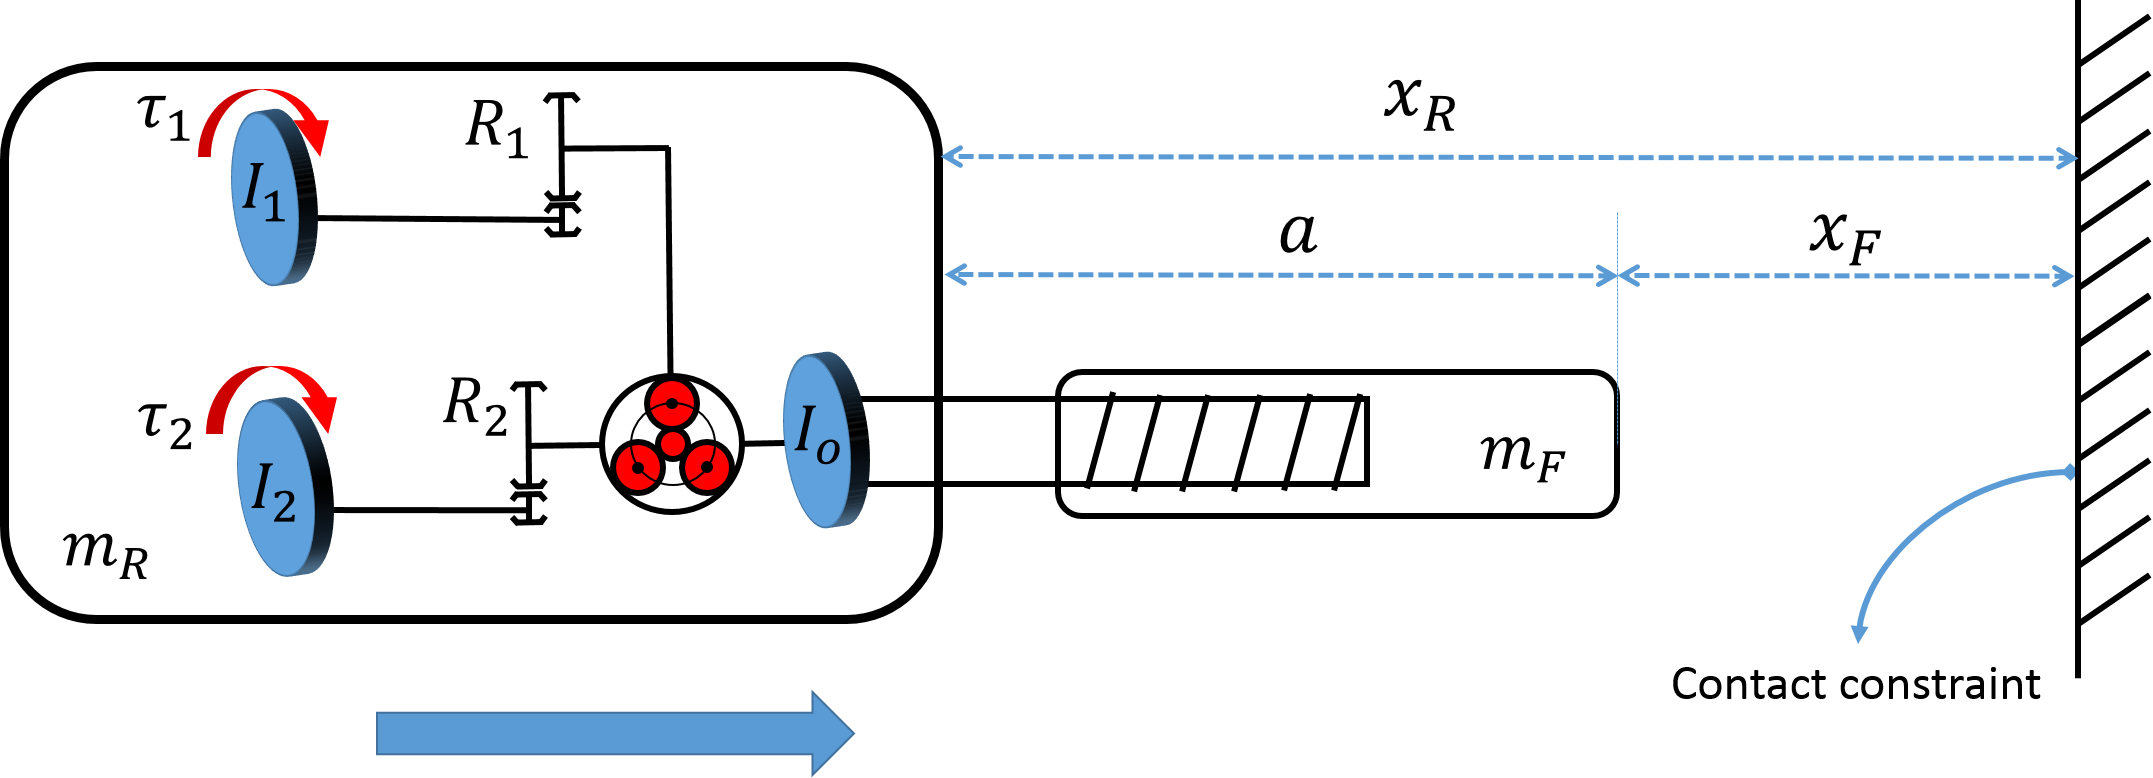
\includegraphics[width=0.95\textwidth]{1dof_landing.png}
	\caption{Simple Robot Landing with a 1-DoF leg equipped with a DSDM}
	\label{fig:1dof_landing}
\end{figure}

However, for the purpose of the high-level control loop, as discussed in Chapter \ref{sec:ControlAndPlanningOfRobotUsingVariableGearRatioActuators}, DSDM actuator can be modeled as variable gear-ratio actuator with two discrete options ($R \in \{R_1,R_2\}$). As illustrated at Fig. \ref{fig:1dof_landing_approx}, in that case the system only have two DoF : absolute velocity of robot base $\dot{x}_R$ and relative leg/actuator velocity $\dot{a}$.

\begin{figure}[htp]
	\centering
		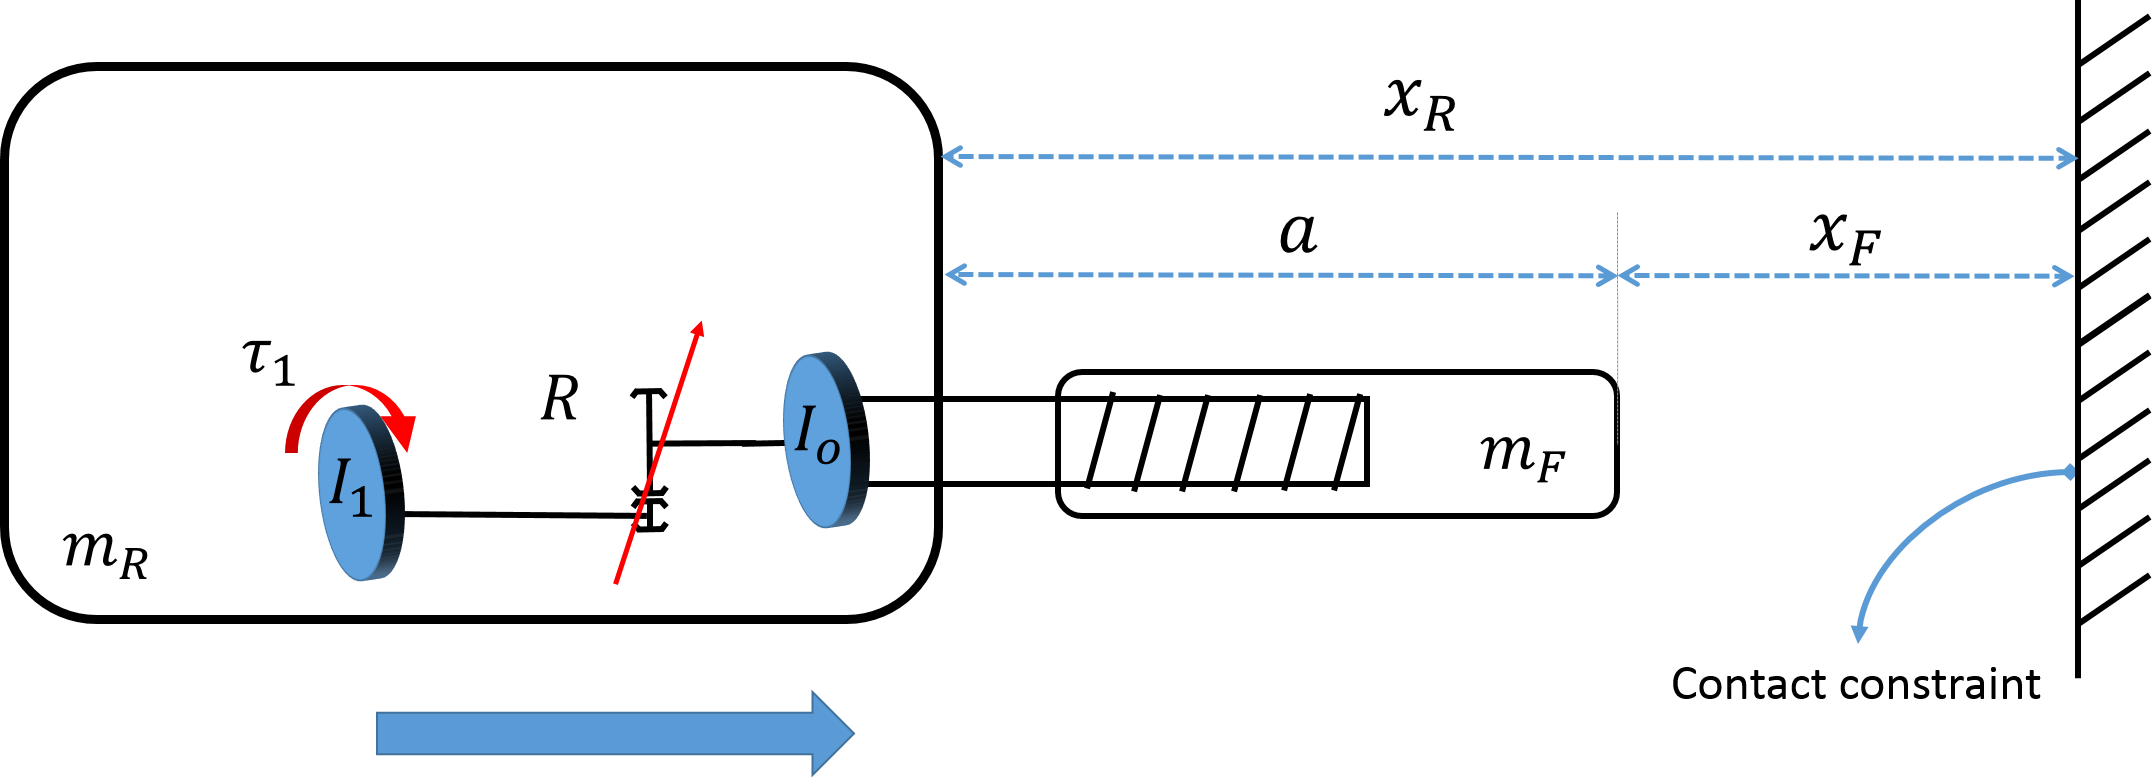
\includegraphics[width=0.95\textwidth]{1dof_landing_approx.png}
	\caption{Simple Robot Landing with a 1-DoF leg equipped with a DSDM}
	\label{fig:1dof_landing_approx}
\end{figure}

%\subsubsection{Kinematic}

The kinematic relationship in the system is described by:
%
\begin{align}
 x_R &= a + x_F \\
 \dot{x}_R &= \dot{a} + \dot{x}_F 
\end{align}
%
and the following variable as used as generalized coordinates:
%
\begin{align}
\dot{\vec{q}} = 
\left[ \begin{array}{c}
\dot{x}_R \\ \dot{a}
\end{array} \right] 
\end{align}


The kinetic energy is given by:
%
\begin{align}
T &= 1/2 \left[ m_R \right] \dot{x}_R^2 + 1/2 \left[ m_F \right] \dot{x}_F^2 + 1/2 \underbrace{\left[ I_o + R^2 I_1 \right]}_{I_a} \dot{a}^2 \\
T &= 1/2 
\left[ \begin{array}{c c}
\dot{x}_R & \dot{a}
\end{array} \right] 
\underbrace{
\left[ \begin{array}{c c}
m_R + m_F & -m_F \\
-m_F      & I_a + m_F
\end{array} \right] }_{H}
\underbrace{
\left[ \begin{array}{c}
\dot{x}_R \\ \dot{a}
\end{array} \right] }_{\dot{\vec{q}}}
\end{align}
%
When the leg is in contact with the ground the constraint is described by:
%
\begin{align}
\phi( \vec{q} )       &= x_R - a = 0 \\
\dot{\phi}( \vec{q} ) &= J_c\vec{\dot{q}}  = 0 \\
J_c                   &= \frac{d \phi}{d\vec{q}} = \left[ \begin{array}{c c} 1 & -1 \end{array} \right]
\label{eq:dsdm_impact_const}
\end{align}
%
The equation of motion is then given by:
%
\begin{align} 
\underbrace{
\left[ \begin{array}{c c}
\scriptsize m_R + m_F & -m_F \\
\scriptsize -m_F      & I_a + m_F
\end{array} \right] }_{H}
\underbrace{
\left[ \begin{array}{c}
\ddot{x}_R \\ \ddot{a}
\end{array} \right] }_{\ddot{\vec{q}}}
+
\underbrace{
\left[ \begin{array}{c c}
0      & 0 \\
0      & b_a 
\end{array} \right] }_{D}
\underbrace{
\left[ \begin{array}{c}
\dot{x}_R \\ \dot{a}
\end{array} \right] }_{\dot{\vec{q}}}
+
\underbrace{
\left[ \begin{array}{c}
-(m_R+m_F)g \\ m_F g 
\end{array} \right] }_{\vec{g}}
=
\underbrace{
\left[ \begin{array}{c}
0 \\ R_1
\end{array} \right] }_{B}
\tau_1
+
\underbrace{
\left[ \begin{array}{c}
1 \\ -1
\end{array} \right] }_{J_c^T}
f_c
\end{align}
%
Those EoM are valid for all possible situations:
%
\begin{align}
&\text{Flight phase:} \quad f_c = 0 \\
&\text{Leg on the ground:} \quad f_c \neq 0 \\
&\text{High-force Mode:} \quad I_a = I_o + R_1^2 I_1 \quad b_a = b_o + R_1^2 b_1 \\
&\text{High-speed Mode:} \quad I_a = I_o + R_2^2 I_2 \quad b_a = b_o + R_2^2 b_2
\end{align}
%
When the robot hit the ground, the impulsive contact force is given by:
%
\begin{align}
\int{  f_c dt } &= - \left( J_c H^{-1} J_c^T \right)^{-1}  J_c \vec{\dot{q}}^- =
\left[ m_F + (\frac{m_R I_a}{m_R + I_a}) \right] \underbrace{(\dot{x}_R^- - \dot{a}^-)}_{\dot{x}_F^-}
\label{eq:dsdm_impact_force}
\end{align}
%
and the associated impulsive change in velocities is given by:
%
\begin{align}
\left[ \begin{array}{c}
\Delta \dot{x}_R \\ \Delta \dot{a}
\end{array} \right]
 &= H^{-1} J_c^T \int{  f_c dt } = \frac{1}{I_a + m_R} \left[ \begin{array}{c}
I_a \\ -m_R
\end{array} \right] \dot{x}_F^-
\label{eq:dsdm_impact_delta}
\end{align}
%

\subsection{Desired Motion}

\subsection{R* controller for the Flight phase}

During the flight phase, there is 2 DoF and only one actuator, the system is thus under-actuated. Moreover, the dynamic of the CoM is completely uncontrollable. The proposed R* algorithm, see Chapter \ref{sec:ControlAndPlanningOfRobotUsingVariableGearRatioActuators}, can still be used to control one out of the two DoF, i.e. using partial feedback linearization instead of full feedback linearization. 

The dynamic of the controllable DoF can be extracted:
\begin{align}
\left[ I_a + \left( \frac{m_F m_R}{m_F + m_R} \right) \right] \ddot{a} + \Bigg[ b_a \Bigg] \dot{a} = R_1 \tau_1
\end{align}
%
and then rearranging to separate extrinsic and intrinsic torques:
%
\begin{align} 
\frac{1}{R}
\underbrace{\left(
\left[ I_o + \left( \frac{m_F m_R}{m_F + m_R} \right) \right] \ddot{a} + \Bigg[ b_o \Bigg] \dot{a}
\right)}_{\tau_E}
+ R
\underbrace{\left(
 I_1 \ddot{a} + b_1 \dot{a}
\right)}_{\tau_I}
= \tau_1
\end{align}
%
Then the R* controller can be used to track a trajectory for the leg $a(t)$:
%
\begin{align} 
\tau_1 &= \frac{1}{R^*} \tau_E( \ddot{a}_R , \dot{a} ) + R^* \, \tau_I( \ddot{a}_R , \dot{a} ) \\ 
& \text{with} \quad R^* = argmin\left[ \tau_1^T \tau_1\right] \\
& \quad \quad \quad R \in \{R_1, R_2\}
\end{align}
%



\subsubsection{Predictive Impact Controller in DSDM Nullspace}


Effect on DSDM actuator.\\
High-level analysis give impulsive behavior of the actuator output DoF:
%
\begin{align}
\Delta \dot{a} = \frac{ \int{\tau_c dt} }{ I_a }  = \frac{-m_R}{I_a + m_R} \dot{x}_F^-
\end{align}
%
Impulsive torque on actuator output:
%
\begin{align}
\int{\tau_c dt} = \frac{-m_R I_a}{I_a + m_R} \dot{x}_F^-
\end{align}
%
Ideal desired M1 velocity before the impact:
\begin{align}
w_{1,d}  = - R_1 \frac{\int{\tau_c dt}}{I_a} =  R_1 \frac{m_R}{I_a + m_R} \dot{x}_F^-
\end{align}
%
Hence if $w_1$ is tracking this target velocity, function of the foot velocity, then after the foot touch the ground:
\begin{align}
w_{1}^+  = 0
\end{align}
and high-force mode can be engaged seamlessly.


\subsection{Ground Phase Control}

The dynamic of the actuated DoF can be extracted:
%
\begin{align}
\left[ I_a + \left( \frac{m_F m_R}{m_F + m_R} \right) \right] \ddot{a} + \Bigg[ b_a \Bigg] \dot{a} = R \tau_1 - \Bigg[ \frac{m_R}{m_R+m_F} \Bigg] f_c
\end{align}
%
The contact force can be computed using eq. \eqref{eq:const_forces}:
%
\begin{align}
f_c = \left( J_c H^{-1} J_c^T \right)^{-1} \left(  J_c H^{-1} [\vec{c} - B \vec{\tau} ] ) \right)
= \frac{m_R}{I_a+m_R} \Bigg[ R \tau - \left(I_a + \frac{I_a m_F}{m_R} + m_F \right) g - b_a \dot{a} \Bigg]
\end{align}
%
For complex robots, the R* algorithm could be implemented by considering the contact $f_c$ as a known term in the EoM, which would be computed online. However here, since the system is simple, it is possible to combine both equations beforehand and get an analytical 1-DoF equation after elimination:
%
\begin{align}
\left[ I_a + m_R \right] \ddot{a} + \left[ b_a \right] \dot{a} = R \tau_1 
\end{align}
%
and then rearranging to separate extrinsic and intrinsic torques:
%
\begin{align} 
\frac{1}{R}
\underbrace{\left(
\left[ I_o + m_R \right] \ddot{a} + \left[ b_o \right] \dot{a}
\right)}_{\tau_E}
+ R
\underbrace{\left(
 I_1 \ddot{a} + b_1 \dot{a}
\right)}_{\tau_I}
= \tau_1
\end{align}
%



\section{Experiments}
\label{sec:case_exp}



